%& C:\Users\RANGAR~1\AppData\Roaming\TikzEdt\TikzEdt\023~1.0\TEMP_H~1
\begin{document}
\pgfplotsset{compat=1.12}
\pgfplotsset{every tick label/.append style={font=\scriptsize}}
  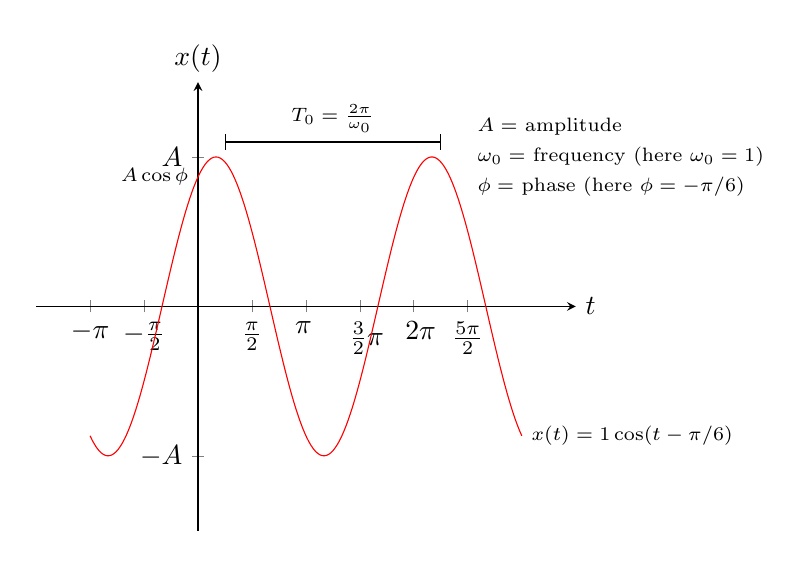
\begin{tikzpicture}
  \def\omwga0{2*pi}
  \def\phase{-30}
    \begin{axis}[
     clip=false,
     xmin=-1.5*pi,xmax=3.5*pi,
     xlabel= $t$,
     ylabel=$ x(t)$,
     ymin=-1.5,ymax=1.5,
     axis lines=middle,
     %axis x line=middle,
     %axis y line=left,
%     axis x line=middle,
     xtick={-3.14, -1.57, 0,1.57,3.14,4.71,6.28, 7.85},
     xticklabels={$-\pi$, $-\frac{\pi}{2}$, $0$, $\frac{\pi}{2}$,$\pi\,$,$\,\,\,\frac{3}{2}\pi$,$\,\,\,2\pi$, $\frac{5\pi}{2}$},
     ytick={-1, 1},
     yticklabels={$\small  -A$, $\small  A$},
     %xticklabel style={anchor=north west}
        x label style={at={(current axis.right of origin)},anchor=west},
        y label style={at={(current axis.above origin)}, anchor=south},
     ]
      \addplot[domain=-pi:3*pi,samples=200,red]{cos(deg(x) + \phase)}
                                node[right,pos=1,font=\footnotesize, black]{\scriptsize $x(t)=1\cos (t - \pi/6)$};


       \draw[|-|] (axis cs: pi/4,1.1) -- (axis cs: 2*pi +pi/4,1.1) node[midway, above] {\scriptsize $T_0=\frac{2\pi}{\omega_0}$};
       \node at (axis cs:0, .8667) [anchor=east] {\scriptsize $A\cos\phi$  };

       \node at (axis cs:2.5*pi, 1.2) [anchor=west] {\scriptsize $A =$ amplitude };
       \node at (axis cs:2.5*pi, 1.0) [anchor=west] {\scriptsize $\omega_0 =$ frequency (here $\omega_0 =1$) };
       \node at (axis cs:2.5*pi, 0.8) [anchor=west] {\scriptsize $\phi =$ phase (here $\phi =-\pi/6$) };
    \end{axis}


  
\usetikzlibrary{calc}
\pgftransformreset
\node[inner sep=0pt,outer sep=0pt,minimum size=0pt,line width=0pt,text width=0pt,text height=0pt] at (current bounding box) {};
%add border to avoid cropping by pdflibnet
\foreach \border in {0.1}
  \useasboundingbox (current bounding box.south west)+(-\border,-\border) rectangle (current bounding box.north east)+(\border,\border);
\newwrite\metadatafile
\immediate\openout\metadatafile=\jobname_BB.txt
\path
  let
    \p1=(current bounding box.south west),
    \p2=(current bounding box.north east)
  in
  node[inner sep=0pt,outer sep=0pt,minimum size=0pt,line width=0pt,text width=0pt,text height=0pt,draw=white] at (current bounding box) {
\immediate\write\metadatafile{\p1,\p2}
};
\immediate\closeout\metadatafile
\end{tikzpicture} 

\end{document}



